%-------- Document Class  ------------------------------------------------------------------------------------------------------------------------------------------------
\documentclass[a4paper,10pt]{report}
\usepackage[a4paper, margin=2.25cm]{geometry}

%-------- Multi-file  ---------------------------------------------------------------------------------------------------------------------------------------------------------
\usepackage{subfiles}

%-------- Preambolo  --------------------------------------------------------------------------------------------------------------------------------------------------
%Per le Figure
\usepackage[english]{babel}
\usepackage{graphicx}

%simboli matematici strani quali unione disgiunta
\usepackage{amssymb}

%Scrivere Sotto i simboli
\usepackage{amsmath}

%Diagrammi Commutativi
\usepackage{tikz}
\usetikzlibrary{matrix}

%Il simbolo di Identità
\usepackage{dsfont}

%Per riflettere i simboli...
\usepackage{graphicx}


%link iNTERNET
\usepackage{hyperref}

%Enumerate with letters
\usepackage{enumerate}

%Slash over letter
\usepackage{cancel}

%Usare bibiliografia bibtex
%\bibliographystyle{plain}

%Danger sign
\usepackage{fourier}

%:=
\usepackage{mathtools}

%http://tex.stackexchange.com/questions/8625/force-figure-placement-in-text
\usepackage{caption}


%subsection numbering
 \setcounter{tocdepth}{3} % if you want all the levels in your table of contents

%Common symbols
%Common math symbols
	%Number fields
		\newcommand{\Real}{\mathbb{R}}
		\newcommand{\Natural}{\mathbb{N}}
		\newcommand{\Relative}{\mathbb{Z}}
		\newcommand{\Rational}{\mathbb{Q}}
		\newcommand{\Complex}{\mathbb{C}}
	
%equality lingo
	%must be equal
		\newcommand{\mbeq}{\overset{!}{=}} 

% function
	%Domain
		\newcommand{\dom}{\mathrm{dom}}
	%Range
		\newcommand{\ran}{\mathrm{ran}}
	

% Set Theory
	% Power set (insieme delle parti
		\newcommand{\PowerSet}{\mathcal{P}}

%Differential Geometry
	% Atlas
		\newcommand{\Atlas}{\mathcal{A}}
	%support
		\newcommand{\supp}{\textrm{supp}}

	
	
%Category Theory
	%Mor set http://ncatlab.org/nlab/show/morphism
%		\newcommand{\hom}{\textrm{hom}}

%Geometric Lagrangian Mechanics
	% Kinematic Configurations
		\newcommand{\Conf}{\mathtt{C}}
	%Solutions Space
		\newcommand{\Sol}{\mathtt{Sol}}
	%Lagrangian class
		\newcommand{\Lag}{\mathsf{Lag}}
	%Lagrangiana
		\newcommand{\Lagrangian}{\mathcal{L}}
	%Data
		\newcommand{\Data}{\mathsf{Data}}
	%unique solution map
		\newcommand{\SolMap}{\mathbf{s}}
	%Classical Observables
		\newcommand{\Obs}{\mathcal{E}}	
	%Phase Space
		\newcommand{\Phase}{\mathcal{M}}	

		\
		
%Peierls (per non sbagliare più)
		\newcommand{\Pei}{Peierls}

%Accented Letters
\usepackage[utf8]{inputenc}

%Temporaneo, Aggiunta della mia classe teorem... Deve diventare un pacchetto!
\input{../Latex-Theorem/TheoremTemplateToninus.tex}
%Common math symbols
	%Number fields
		\newcommand{\Real}{\mathbb{R}}
		\newcommand{\Natural}{\mathbb{N}}
		\newcommand{\Relative}{\mathbb{Z}}
		\newcommand{\Rational}{\mathbb{Q}}
		\newcommand{\Complex}{\mathbb{C}}
	
%equality lingo
	%must be equal
		\newcommand{\mbeq}{\overset{!}{=}} 

% function
	%Domain
		\newcommand{\dom}{\mathrm{dom}}
	%Range
		\newcommand{\ran}{\mathrm{ran}}
	

% Set Theory
	% Power set (insieme delle parti
		\newcommand{\PowerSet}{\mathcal{P}}

%Differential Geometry
	% Atlas
		\newcommand{\Atlas}{\mathcal{A}}
	%support
		\newcommand{\supp}{\textrm{supp}}

	
	
%Category Theory
	%Mor set http://ncatlab.org/nlab/show/morphism
%		\newcommand{\hom}{\textrm{hom}}

%Geometric Lagrangian Mechanics
	% Kinematic Configurations
		\newcommand{\Conf}{\mathtt{C}}
	%Solutions Space
		\newcommand{\Sol}{\mathtt{Sol}}
	%Lagrangian class
		\newcommand{\Lag}{\mathsf{Lag}}
	%Lagrangiana
		\newcommand{\Lagrangian}{\mathcal{L}}
	%Data
		\newcommand{\Data}{\mathsf{Data}}
	%unique solution map
		\newcommand{\SolMap}{\mathbf{s}}
	%Classical Observables
		\newcommand{\Obs}{\mathcal{E}}	
	%Phase Space
		\newcommand{\Phase}{\mathcal{M}}	

		\
		
%Peierls (per non sbagliare più)
		\newcommand{\Pei}{Peierls}	%Common symbols
\usepackage{glossaries}

\makenoidxglossaries

%How to:
%affinchè la voce venga printata nella lista va prima chiamata nel testo come e.g. \gls{Bundle}
%ricordarsi di chiamarlo almeno una volta così, dopo usare il command per evitare il ripetuto hyperref
% anche se si potrebbe evitare visto che il quadratino del link non dovrebbe apparire in stampa

%Advanced Differential Geometry
\newglossaryentry{Bundle}%
{%
	name={\ensuremath{E = (E,\pi , M;Q)}},
	description={ Fiber Bundles $\pi: E\rightarrow M$ with typical fiber $Q$},
    sort={B}
}

\newglossaryentry{Sections}%
{%
	name={\ensuremath{\Gamma^\infty(E)}},
	description={ Smooth sections on the bundle $E$.},
    sort={S}
}


%Geometric Lagrangian Mechanics
	% Kinematic Configurations
	\newglossaryentry{Conf}%
	{%
		name={\ensuremath{\Conf}},
		description={ Kinematic Configurations set}
	}

	%Solutions Space
	\newglossaryentry{Sol}%
	{%
		name={\ensuremath{\Sol}},
		description={ Dynamic Configurations set}
	}

		
	%Lagrangian class
		\newglossaryentry{Lag}%
	{%
		name={\ensuremath{\Lag}},
		description={ Set of Lagrangian densities.}
	}
		
	%Lagrangiana
	\newglossaryentry{Lagrangian}%
	{%
		name={\ensuremath{\Lagrangian}},
		description={ Lagriangian density of the system.}
	}
		
	%Data
	\newglossaryentry{Data}%
	{%
		name={\ensuremath{\Data}},
		description={ Inital Data set.}
	}
		
	%unique solution map
	\newglossaryentry{SolMap}%
	{%
		name={\ensuremath{\SolMap}},
		description={ Map that map a fixed initial data to the unique solution.}
	}
		
	%Classical Observables
	\newglossaryentry{Obs}%
	{%
		name={\ensuremath{\Obs}},
		description={ Set of all classical observables.}
	}

	%Phase Space
	%Classical Observables
	\newglossaryentry{Phase}%
	{%
		name={\ensuremath{\Phase}},
		description={ Phase space.}
	}



\hyphenation{gua-ran-te-ed}
\hyphenation{Ha-da-mard}
\hyphenation{Rieman-nian}
\pagestyle{empty}

%Temporaneo, Aggiunta della mia classe teorem... Deve diventare un pacchetto!
\input{../../Latex-Theorem/TheoremTemplateToninus.tex}

%---------------------------------------------------------------------------------------------------------------------------------------------------------------------
\title{Demystification of Peierels Brackets construction}
\author{Antonio Michele Miti}
\date{\vspace{-5ex}} % workaround to omit the Date !

%\/\/\/\/\/\/\/\/\/\/\/\/\/\/\/\/\/\/\/\/\/\/\/\/\/\/\/\/\/\/\/\/\/\/\/\/\/\/\/\/\/\/\/\/\/\/\/\/\/\/\/\/\/\/\/\/\/\/\/\/\/\/\/\/\/\/\/\/\/
\begin{document} %\/\/\/\/\/\/\/\/\/\/\/\/\/\/\/\/\/\/\/\/\/\/\/\/\/\/\/\/\/\/\/\/\/\/\/\/\/\/\/\/\/\/\/\/\/\/\/\/\/\/\/\/\/\/\/\/\/\/\/

	%\maketitle
	\section*{Demystification of Peierels Brackets construction}

	%Abstact dynamical system
	\begin{definition}[Dynamical System]\label{Def:AbstracDynamicalSystem}
		%Corretto da CD prima era "Evolutive system"
		We call \emph{abstract dynamical system}
		a pair $(E,P )$ composed of:
		\begin{compactitemize}
			\item $E \xrightarrow{\pi} M$ \\
			smooth fiber bundle of typical fiber $Q$ on  manifold $M$, called \emph{"configuration bundle"}.
			\item	$ P : \Gamma^\infty(E) \rightarrow \Gamma^\infty(E)$ \\
			differential operator %\\  operator called \emph{"motion operator"}
			in the sense that it is represented by a linear combination of partial derivative in every local chart.
			%In cascione ho raccolto la discussione su questo punto
		\end{compactitemize}
	\end{definition}

	\begin{figure}[h!]
		\centering
		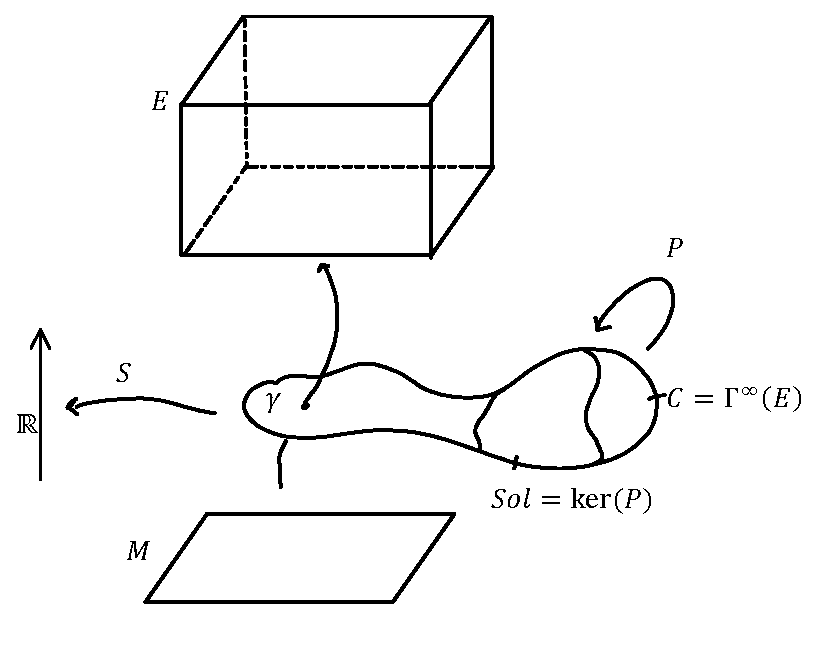
\includegraphics[width=0.5\textwidth]{../Pictures/AbstractFieldTheory}
	\end{figure}

	\begin{definition}[Space of kinematics (off-shell) configurations]
		We call:
		\begin{displaymath}
			\gls{Conf} \coloneqq \Gamma^\infty(M,E)
		\end{displaymath}
		the space of kinematic configurations.
	\end{definition}

	\begin{definition}[Space of Dynamics (on-shell) configurations]\label{Def:SolSpace}
		We call
		\begin{displaymath}
			\gls{Sol} \coloneqq \ker(P) = \left\{\left. \gamma \in \Conf \quad\right\vert  R(P)\left(f\right) = 0 \quad \forall \textrm{local chart representation}\right\}
		\end{displaymath}
		where we have denoted respectively as $R(P)$ and $f$ the local chart representation (as in Eq. \ref{Def:LocalChartRepresentation}) of $P$ and $\gamma$ on the same chart.\\
		This is the subset of $\Conf$ containing all the smooth solutions of the motion equations corresponding to the  dynamical operator:
		\begin{displaymath}
			P: \Conf \rightarrow \Conf
		\end{displaymath}
	\end{definition}

	% Abstract Lagrangean system
	\begin{definition}[Lagrangian System ( of $r$-th order)]
		We call \emph{Lagrangian system} of $r$-th order the
		pair $(E, \mathcal{L} )$ composed of:
		\begin{compactitemize}
			\item $E \xrightarrow{\pi} M$ \\smooth fiber bundle of typical fiber $Q$ on the oriented pseudo-Riemannian manifold $(M,g,\mathfrak{o})$ called \emph{"configuration bundle"}.
			\item	$ \gls{Lagrangian} : J^r E \rightarrow \wedge^m T^*M$ \\bundle-morphism from the r-th Jet Bundle (see Section \ref{Sect:JetBundles}) to  the top-dimensional form bundle over the base manifold $M$  called \emph{"Lagrangian density"} or simply \emph{"Lagrangian"} of r-th order.
		\end{compactitemize}
	\end{definition}

	\begin{definition}[Lagrangian Densities on the bundle $E$]\label{Def:LagrangianDensities}
		We denote the set of all \emph{Lagrangian densities} (of $r-$th order) on the bundle $E$ as:
		\begin{displaymath}
			\gls{Lag}^r (E) \coloneqq \hom\biggr(J^r E,\quad \bigwedge^m( T^*M)\biggr)  \cong \big\{f:\Gamma^\infty(J^r E) \rightarrow \Omega^m(M)  \big\}
		\end{displaymath}
		(where $\Omega^m(M)$ is the common name for $\Gamma^\infty \big( \bigwedge^m( T^*M) \big)$ in the context of Grassmann algebras.)\\
		The equivalence states the fact that a bundle-morphism induces a map between the sections.
	\end{definition}
	%this choice fix the "Dynamical identity" of the considered system. (Correzione CD)
	\begin{proposition}
		$\Lag^r(E)$ has an vector space structure inherited by the linear structure of $\Omega(M)$.
	\end{proposition}

	\begin{definition}[Lagrangian functional]\label{Def:LagrangianFunctionals}
		We call \emph{Lagrangian functional} a map :
		%Is a functional on $\Conf$ with values on regular distribution over M associated to the generic $\Lagrangian \in \Lag$.	(Correzione CD)
		\begin{displaymath}
			\mathcal{O}_\Lagrangian : \Conf \rightarrow D'(M)
		\end{displaymath}
		where  $D'(M)$ is the space of regular distribution over $M$, %\big( C^\infty_0(M) \big)' io lo avevo indicato come il duale delle funzioni di test
		whose action on any configuration $\phi \in \Conf$, evaluated on the test-function $f \in C^\infty_0(M)$, it is given by:
		\begin{displaymath}
			\mathcal{O}_\Lagrangian [\phi] (f) = \int_M \Lagrangian [\phi] f \textrm{d}\mu
		\end{displaymath}
	\end{definition}

	\begin{definition}[Euler-Lagrange operator]
		We call \emph{Euler-Lagrange operator}, the  differential operator
		\begin{displaymath}
			Q_\chi : \Conf \rightarrow \Conf
		\end{displaymath}
		relative to the Lagrangian density $\chi \in \Lag^1(E)$, such that:
		\begin{equation}
			Q_\chi (\gamma) = \Biggr( \nabla_\mu \biggr( \frac{\partial \chi}{\partial(\partial_\mu \phi)} \biggr\vert_\gamma \biggr) - \frac{\partial \chi}{\partial \phi}\biggr\vert_\gamma \Biggr) \qquad \forall \gamma \in \Conf
		\end{equation}
		Where $\nabla_\mu$ is the covariant derivative corresponding to the background metric $g$.
		\footnote{$\frac{\partial \chi}{\partial(\partial_\mu \phi)}$ has the be intended as the Lagrangian density constructed differentiating $\chi(\phi, \partial_\mu)$ as an ordinary function, treating its functional entries as an usual scalar variable.}
	\end{definition}

	\subsection{TODO: Peirels constuction lingo}

	\begin{definition}[Disturbance]
		By \emph{"disturbance"} we mean a time-compact supported Lagrangian density $\chi \in \Lag$\footnote{I.e. the top form $\chi(\phi)$ is time-compact supported for all $\phi \in \Conf$.} which acts as a perturbation on the Lagrangian of the system:
		\begin{displaymath}
			\Lagrangian \rightsquigarrow \Lagrangian' = \Lagrangian + \epsilon\cdot \chi
		\end{displaymath}
		where $\epsilon$  is a real modulation parameter.
		Recalling that $\Lag$ is linear we have that $\Lagrangian'$ is still a suitable Lagrangian of the system.
	\end{definition}

	\begin{definition}[Disturbed Motion equation under a Disturbance (Jacobi Equation)]
		\begin{equation}\label{PeierlJacobiEqLin}
			\Rightarrow P \eta = - Q_\chi \phi(x)
		\end{equation}
		called \emph{Jacobi Equation}.
		It yelds the pertubation to apply to a fixed configuration:
		\begin{displaymath}
			\phi'(x) = \phi(x) + \epsilon \eta(x) \in \Conf
		\end{displaymath}
		such that:
		\begin{displaymath}
			\begin{cases}
				P_\epsilon \phi'(x) &= o(\epsilon)  \\
				P \phi(x) &= 0
			\end{cases}
		\end{displaymath}
	\end{definition}

	\begin{definition}[Effect Operator]
		Considering an arbitrary continuous\footnote{The precise notion of continuity require the specification of a (infinite dimensional) manifold structure on $\Conf$.} functional $B: \Conf \rightarrow \Real$ (not necessarily linear) we can define the effect of a perturbation on the values of $B$\cite[pag. 5]{Marolf1993} as a map:
		\begin{displaymath}
			\gls{EffectOp} : C^1(\Conf,\Real) \rightarrow C^1(\Conf,\Real)
		\end{displaymath}
		\begin{equation}\label{EffectOperator}
			\EffectOp_\chi^\pm B ( \phi_0)
			\coloneqq \lim_{\epsilon \rightarrow 0}
			\biggr( \frac{B(\phi_\epsilon^\pm) - B (\phi_0)}{\epsilon} \biggr)
		\end{equation}
	\end{definition}

	\begin{definition}[Peierls Bracket]
 		The binary function
		\begin{displaymath}
			\{\cdot,\cdot\}:\Lag_{\textrm{tc}} \times \Lag_{\textrm{tc}} \rightarrow \Real 	
		\end{displaymath}
		such that
		\begin{equation}\label{AbstractPeierlsBracket}
				\{\chi, \omega \}(\phi_0) \coloneqq \EffectOp_\chi^- \mathcal{O}_\omega (\phi_0) - \EffectOp_\chi^+ \mathcal{O}_\omega(\phi_0)
		\end{equation}	
	\end{definition}
	
	
	\subsection{TODO: Symplectic space of field-theoretic systems.}
	\begin{remark}
	questo lo devo dire  a parole o scriverlo?
	\begin{itemize}
		\item linear system
		\item green hyperbolic dynamics
		\item globally hyperbolic spacetime based sections
	\end{itemize}
	\end{remark}
	
	\begin{definition}[Configuration Pairing]
		The \emph{pairing} between two sections is defined as:
   			\begin{equation}\label{Def:Pairing}
			(X,Y) = \int_M <X,Y>_x d\mu(x)
			\end{equation}
			where $d\mu = d\textrm{Vol}_\mu$ is the volume form induced by the metric and the orientation on $M$
			under the additional constraint:
  				(The definition is well posed only in:)
 			\begin{displaymath}
				\dom\big( (\cdot, \cdot) \big) =
				\big\{(X,Y) \in \Gamma^\infty(E) \times \Gamma^\infty(E) \; \big\vert \,  <X,Y>_x \in L^1(M,\mu)\big \}
			\end{displaymath}
	\end{definition}
	
	\begin{definition}[Pre-Observable]
		They are defined as a class of \emph{"off-shell"} functionals on $\Conf$:
		
		\begin{displaymath}
			\Obs_0 \coloneqq \biggr\{ F_f: \Conf \ni \phi \mapsto ( f, \phi) \in \Real \quad
			\left\vert\quad  f \in \Gamma_0^\infty(E) \right.	\biggr\}
		\end{displaymath}
		This can be seen as the range of the linear map:
		\begin{displaymath}
			F: \Gamma_0^\infty \rightarrow \Obs_0
		\end{displaymath}
		which associates to any section $f\in \Gamma_0^\infty(E)$ the linear functional
		$F_f(\cdot) = (f,\cdot) :\Conf \rightarrow \Real$.\\
	\end{definition}
	
	\begin{definition}[Classical Observable]
  					Due to the degeneracy of the map $F^\Sol$, % it is clear that
   					$\Obs_0^\Sol$ can not be a good set of classical observables.\\
   					Being the kernel known, we can identify all the elements that posses the same corresponding functional:
   					\begin{displaymath}
   						[f] = \big\{f + P g \quad\vert\: g \in \Gamma_0\big\}
   					\end{displaymath}
   					It is natural then to define the classical observables as the quotient space:
   									\begin{displaymath}
   										\Obs \coloneqq \frac{\Obs_0^\Sol}{N}
   									\end{displaymath}

   					Finally, the mapping between these equivalence classes can be easily defined :\\
   					$\forall [f] \in \frac{\Gamma_0}{P\Gamma_0}$ we build the functional $F_{[f]} : \Sol \rightarrow  \Real$ such that:
   					\begin{displaymath}
   						F_{[f]} (\phi) = F_f(\phi) \qquad \forall \phi \in \Sol , \forall f \in [f]
   					\end{displaymath}
   					This functional is well-defined, \textit{i.e.} the expression is independent from the choice of the representative, only on $\Sol$.
   					The reason is that if $\phi \in \Conf \setminus \Sol$, then $F_f(\phi)$ is different for each choice of the representative $f \in [f]$.
   					%From that,
   					This construction is said to " implement the  on-shell condition at the level of functionals".

   					In conclusion the mapping:
   					\begin{displaymath}
   						\frac{\Gamma_0}{P \Gamma_0}  \xmapsto{\quad F \quad} \Obs = F \big( \frac{\Gamma_0}{P \Gamma_0}\big)
   					\end{displaymath}
   					,between suitable equivalence classes  and linear functionals on $\Sol$, guarantees:
   					\begin{itemize}
   						\item a faithful representation since $F$ is bijective.
   						\item the separability condition, a fortiori of separability properties of $\Obs_0^\Sol$.
   					\end{itemize}
   					From now on we will identify these two spaces:
   					\begin{displaymath}
   						\Obs \simeq 	\frac{\Gamma_0}{P \Gamma_0}
   					\end{displaymath}
   					in view of the bijectivity of $F$.
	\end{definition}
	
	\begin{definition}[PreQuantum Symplectic Space]
	todo...
	\end{definition}
	\begin{proposition}
		this structure correspond to a suitable domain restriction of the peierls brackets
	\end{proposition}

\end{document} %\/\/\/\/\/\/\/\/\/\/\/\/\/\/\/\/\/\/\/\/\/\/\/\/\/\/\/\/\/\/\/\/\/\/\/\/\/\/\/\/\/\/\/\/\/\/\/\/\/\/\/\/\/\/\/\/\/\/\/\
%\/\/\/\/\/\/\/\/\/\/\/\/\/\/\/\/\/\/\/\/\/\/\/\/\/\/\/\/\/\/\/\/\/\/\/\/\/\/\/\/\/\/\/\/\/\/\/\/\/\/\/\/\/\/\/\/\/\/\/\/\/\/\/\/\/\/\/\/\/
